\documentclass[letterpaper,titlepage]{article}
\usepackage{Amish_Style}

\newcommand{\incfig}[1]{%
    % \def\svgwidth{\columnwidth}
    \import{./figures/}{#1.pdf_tex}
}

\addbibresource{bibliography.bib} % Imports bibliography file

% Write this paper as if it is my dissertation and then if I want to publish it, then prune it to be a succint paper
% \title{Computation of Persistence Homology Using the Delaunay-Rips Complex: An efficient family of simplicial complexes for topological data analysis}
% \author{Amish Mishra and Francis Motta}
% \date{\today}

\begin{document}

\begin{center}
    \Large
    \textbf{Computation of Persistent Homology Using the Delaunay-Rips Complex}
        
    \vspace{0.4cm}
    \large
    An efficient family of simplicial complexes for topological data analysis
        
    \vspace{0.4cm}
    \textbf{Amish Mishra and Francis Motta}
       
    \vspace{0.9cm}
    \textbf{Abstract}
\end{center}
Topological Data Analysis is an emerging area rooted in theories from Algebraic Topology, which enables researchers to extract discriminating geometric and topological features from data. We give an overview of some of the popular methods of extracting features from point-cloud data, which first requires one to construct a 1-parameter family of spaces on the data using the geometry of the cloud. We demonstrate their benefits and shortcomings and introduce a new, more efficient construction that we name the Delaunay-Rips Complex. We justify conditions on the data that guarantee stability of our method when computing persistent homology. Aided by intuitive examples, we also provide an empirical run-time comparison of the two existing methods with our new algorithm on the computation of the persistence diagrams of some synthetic data sets.



\section{Introduction}
Welcome to our paper!

\section{Background}

\subsection{Topological Data Analysis}
    We are living in an information age where data-driven decision making is a huge area of interest. With so much data at our hands, many questions naturally arise.
    \begin{itemize}
        \item How do we extract relevant information from the data? \item How do we even know what is relevant and what is not? 
        \item If we are unable to visualize large quantities of data, especially data in high dimensions, then how do we know what sort of data set we are inspecting? 
        \item Further, how can we compare information extracted from one data set with another?
    \end{itemize}
    These are the sorts of difficult and fascinating questions tackled in the field of Topological Data Analysis (TDA). From the name itself, TDA hints at leveraging ideas borrowed from topology with data analysis techniques to measure and quantify qualitative features of data. At a more nuanced level, TDA appears as the child of Algebraic Topology, Computer Science, Statistics, Data Analysis, and Computational Geometry. Results from each field have found beautiful applications in TDA and have shed new light on applicability of theoretical results from mathematics.
    
    
\subsection{Simplicial Complexes}
    The idea behind extracting topological features from a given point-cloud requires there to be a method of assigning some sort of ``shape" to the data. Only then are we able to study its associated topological properties. The scenario we face is that we have a finite dimensional metric space out of the point-cloud that we need to assign a shape to. With the human eye, we may be able to make out some appropriate surface our data set can live on. However, this situation pokes at a fundamental question that arises when computing: how can we get a computer to do what a human can do? We need to introduce the idea of a \textit{simplicial complex}, a computational efficient way for a computer to build a surface onto a data set.
    
    \begin{defn}
        A simplicial complex is a collection $K$ of non-empty subsets of a set $K_0$ such that $\{v\} \in K$ for all $v \in K_0$, and if $\sigma \in K$ then $\tau \in K$ for all $\tau \subseteq \sigma$. The elements of $K_0$ are called vertices of $K$, and the elements of $K$ are called simplices. Additionally, we say that a simplex has dimension $p$ or is a $p$-simplex if it has cardinality of $p+1$. We use $K_p$ to denote the collection of $p$-simplices. The $k$-skeleton of $K$ is the union of the sets $K_p$ for all $p \in \{0,1,\dots,k\}$. If $\tau$ and $\sigma$ are simplices such that $\tau \subset \sigma$, then we call $\tau$ a face of $\sigma$, and we say that $\tau$ is a face of $\sigma$ of codimension $k'$ if the dimensions of $\tau$ and $\sigma$ differ by $k'$. The dimension of $K$ is defined as the maximum of the dimensions of its simplices. A map of simplicial complexes, $f: K \to L$, is a map $f: K_0 \to L_0$ such that $f(\sigma) \in L$ for all $\sigma \in K$. \cite{Edelsbrunner}
    \end{defn}
    
\subsection{Simplicial Homology}

\subsection{Vietoris-Rips Complex} \label{rips}
One of the simplest ways to build a complex on a data set $X$ is by considering the pairwise distance between the points. The approach described here is an algorithmic, bottom-up approach that adds higher and higher dimensional simplices to the complex for a fixed scale. For a given scale $\varepsilon>0$, if $d(x,x')\leq 2\varepsilon$ for $x,x' \in X$, then we add the edge between $x$ and $x'$ into our complex. Once all of the edges are added, we add the higher dimensional simplices if their faces are already in the complex. That is, we add the $k$-simplex $\sigma = \{x_0,x_1,\dots,x_k\}$ to the complex if every subset $u \subset \sigma$ is already in the complex. Formally, we define the Vietoris-Rips complex \cite{Roadmap} for scale $\varepsilon>0$ 
$$VR_{\varepsilon}(X) = \{\sigma \subseteq X\ |\ d(x,x') \leq 2\varepsilon,\ \forall x,x' \in \sigma\}.$$

\subsection{Delaunay Triangulation}
Although the Vietoris-Rips complex is simple to implement, constructing it on data sets with large numbers of points results in computation drawback. As the scale increases, we see that adding certain simplices does not affect the homology of the point cloud. We need some way to ``weed" out these extraneous simplices as we construct our complex to increase computational efficiency. Turning to a tool of Computational Geometry, we incorporate the Delaunay Triangulation in our construction. Our definition is adapted from ``A roadmap for the computation of persistent homology"\cite{Roadmap}. Assume our data $X$ lives in the space $\R^n$. Let $x \in X$. We define
$$V_x = \{p \in \R^d\ |\ d(p,x) \leq d(p, x')\ \forall x' \in X\}.$$
Each $V_x$ is called a Voronoi cell. Note that $\{V_x\}_{x \in X}$ forms a cover of $\R^n$. This cover is known as the Voronoi decomposition of $\R^n$ with respect to $X$. To construct the Delaunay triangulation from this cover, we connect $x,x' \in X$ with an edge if $V_x$ and $V_{x'}$ are neighbors (that is, the Vornoi cells share a wall). When the points in $X$ are in general position, this gives us a graph (1-skeleton) on $X$ that is known as the Delaunay Triangulation. Formally, we define \cite{Edelsbrunner}
$$Del(X) = \{\sigma \subset X\ |\ \bigcap_{u \in \sigma} V_u \neq \emptyset\}.$$
We will use $Del(X)$ as the underlying graph structure when defining the Delaunay-Rips complex in section \ref{del-rips:def}.

As an alternate defintion to the Delaunay Triangulation that we will employ in section \ref{stability}, we have the following

\begin{defn}
For a set $X$ of points in $\R^d$, a Delaunay triangulation is a triangulation $DT(X)$ such that no point in $X$ is inside the circum-hypersphere of any simplex in $DT(X)$. 
\end{defn}

\subsection{Persistence}


\section{Delaunay-Rips Complex}
\subsection{Definition and Construction} \label{del-rips:def}
The Delaunay-Rips complex is our alternative method of building a complex on a data set $X$. The idea is similar to the construction of the Delaunay-\u Cech complex defined in \cite{Bauer_2016}. Delaunay-Rips utilizes the conceptual simplicity of the Vietoris-Rips complex while cutting down on the number of high dimensional and extraneous simplices. This computational speed-up is by virtue of using the Delaunay Triangulation as the ``backbone" of building the Vietoris-Rips complex on $X$. The idea is that we build the Vietoris-Rips complex on $X$ but only add edges if the edges occur in the Delaunay 1-skeleton of the point cloud. The higher dimensional $k$-simplices are then added the traditional way they are in section \ref{rips}. Formally, we define the Delaunay-Rips Complex for a given scale $\varepsilon>0$
$$DR_{\varepsilon}(X) = \{\sigma \subseteq Del(X)\ |\ d(x,x') \leq 2\varepsilon,\ \forall x,x' \in \sigma\}.$$


\subsection{Example Data Set}
\begin{enumerate}
    \item Demonstrate construction on a small data-set (5-8 point data-set).
\end{enumerate}
% Rotate 90 degrees counter-clockwise and put them on a line
\begin{figure}[ht!]
    \centering
        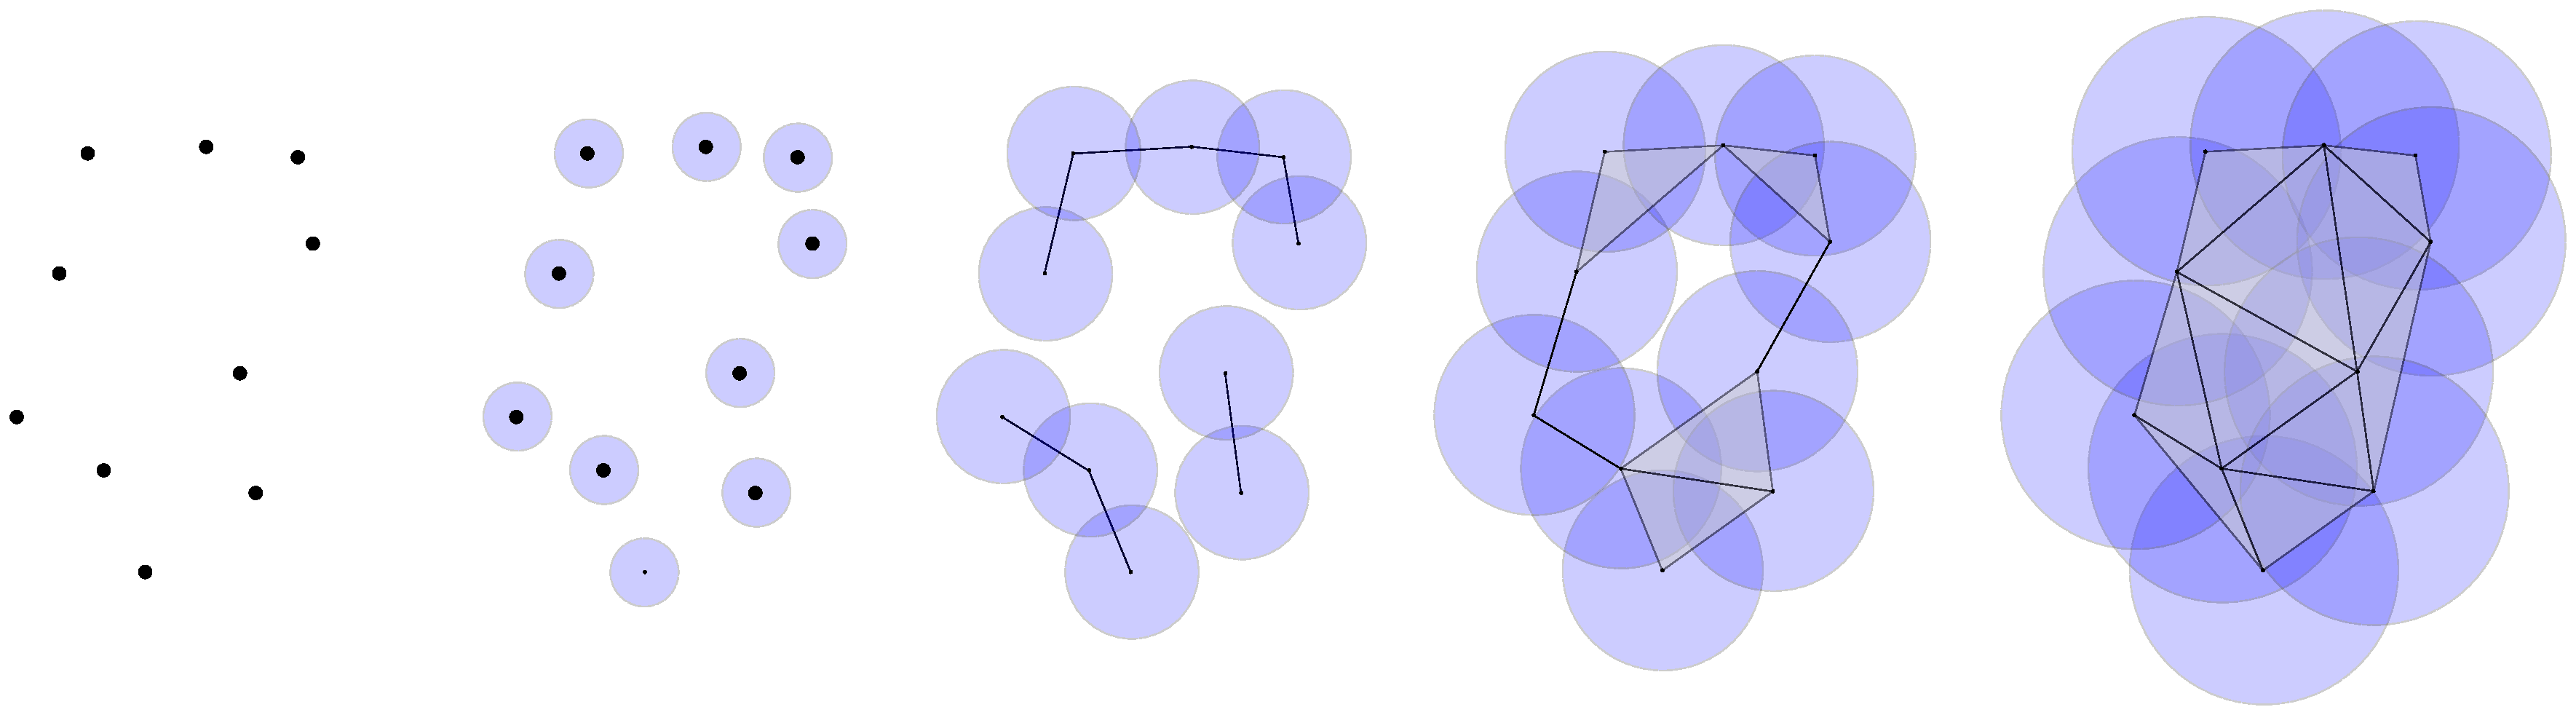
\includegraphics[width=1.0\textwidth]{./figures/test.pdf}
    %\def\svgwidth{0.3\textwidth}
    %\begin{subfigure}[b]{\textwidth}
    %    \incfig{del_rips_construction_ex0}
    %\end{subfigure}
    %\hfill
    %\def\svgwidth{0.3\textwidth}
    %\begin{subfigure}[b]{\textwidth}
    %    \incfig{del_rips_construction_ex1}
    %\end{subfigure}
    %\hfill
    %\def\svgwidth{0.3\textwidth}
    %\begin{subfigure}[b]{\textwidth}
    %   \incfig{del_rips_construction_ex2}
    %\end{subfigure}
    %\def\svgwidth{0.3\textwidth}
    %\begin{subfigure}[b]{\textwidth}
    %    \incfig{del_rips_construction_ex3}
    %\end{subfigure}
    %\hfill
    %\def\svgwidth{0.3\textwidth}
    %\begin{subfigure}[b]{\textwidth}
    %    \incfig{del_rips_construction_ex4}
    %\end{subfigure}
    % \hfill
    % \begin{subfigure}[b]{0.2\textwidth}
    %     \incfig{del_rips_construction_ex1}
    % \end{subfigure}
    % \hfill
    % \begin{subfigure}[b]{0.2\textwidth}
    %     \incfig{del_rips_construction_ex2}
    % \end{subfigure}

    % \begin{subfigure}[b]{0.2\textwidth}
    %     \incfig{del_rips_construction_ex3}
    % \end{subfigure}

    % \begin{subfigure}[b]{0.2\textwidth}
    %     \incfig{del_rips_construction_ex4}
    % \end{subfigure}
    \caption{Example of constructing Delaunay-Rips complex on 10 points in $\R^2$.}
    % \label{fig:circumcenter}
\end{figure}



\subsection{Run-time Analysis Comparison}
In this section, we immediately show some empirical results of the performance of computing persistence using the Delaunay-Rips filtration on varying datasets. The runtimes are measured as the time between the data set being inputed into the corresponding algorithm and the persistence diagram being produced.
\begin{figure}[ht]
    \centering
    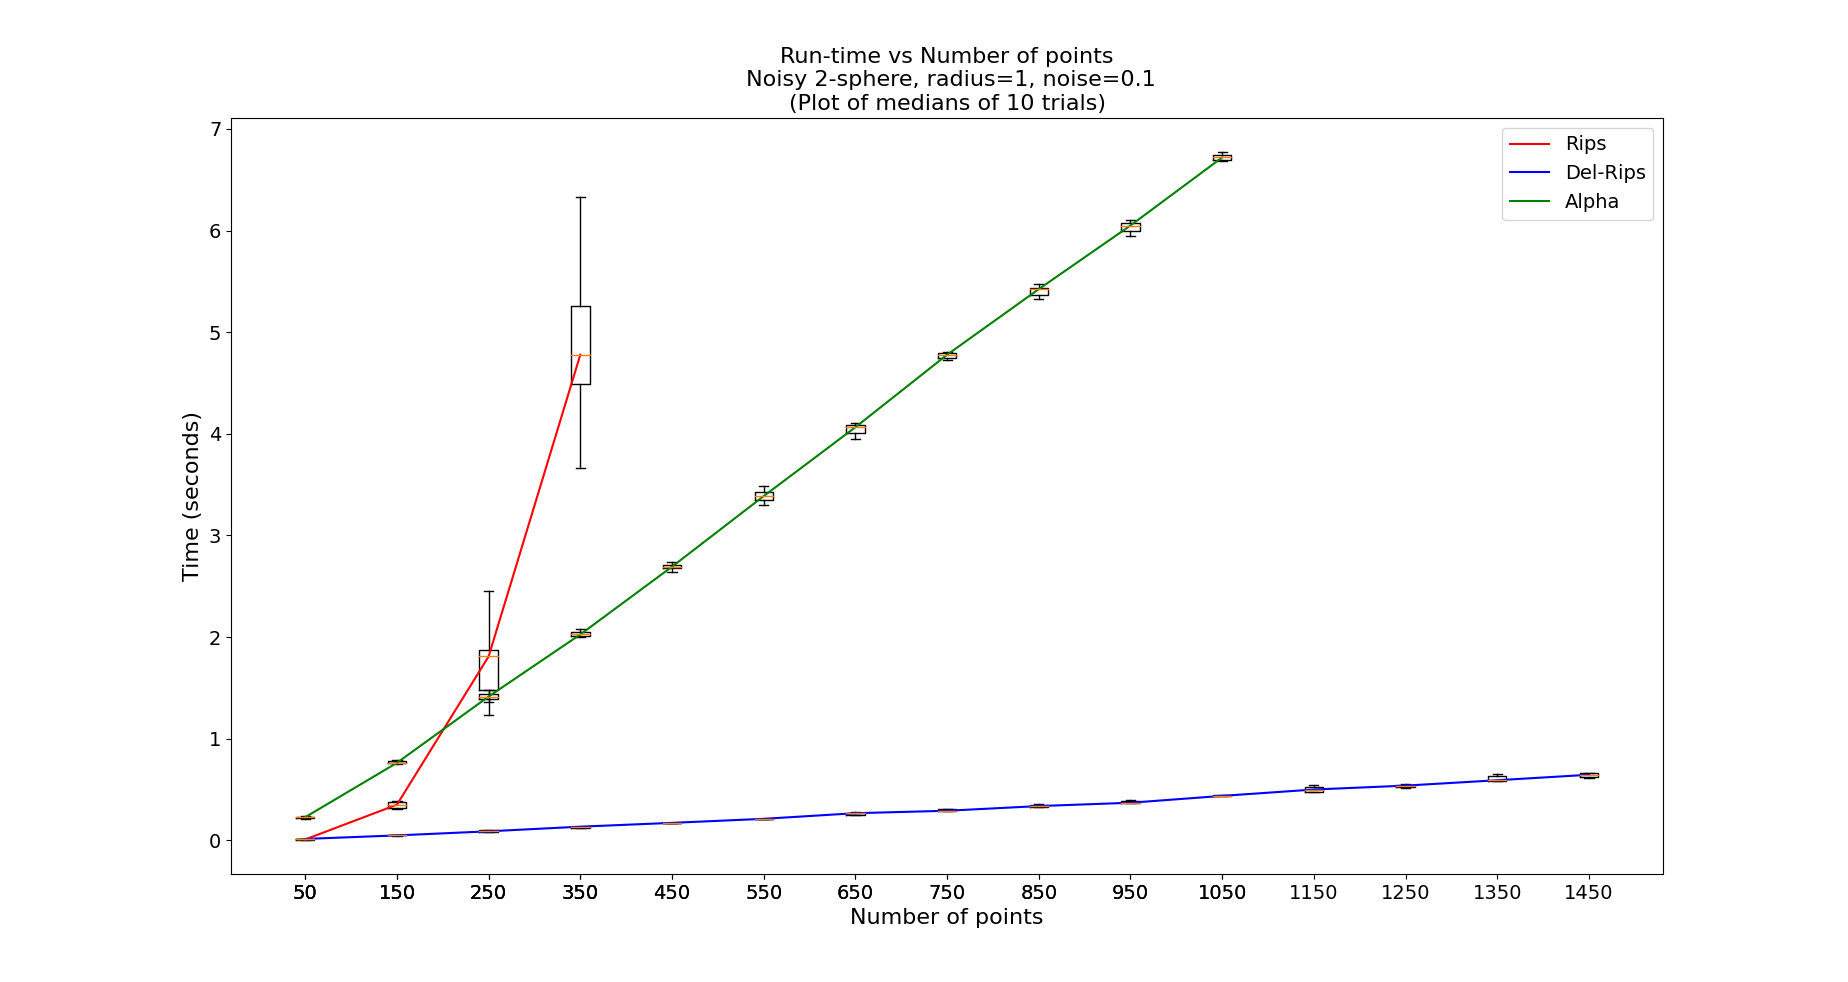
\includegraphics[width=\columnwidth]{./figures/runtime_pts_7sec_cap_3.png}
    \caption{Runtime comparison of Rips, Alpha, and Delaunay-Rips as number of points are increased.}
    \label{fig:runtime_pts}
\end{figure}

\begin{figure}[ht]
    \centering
    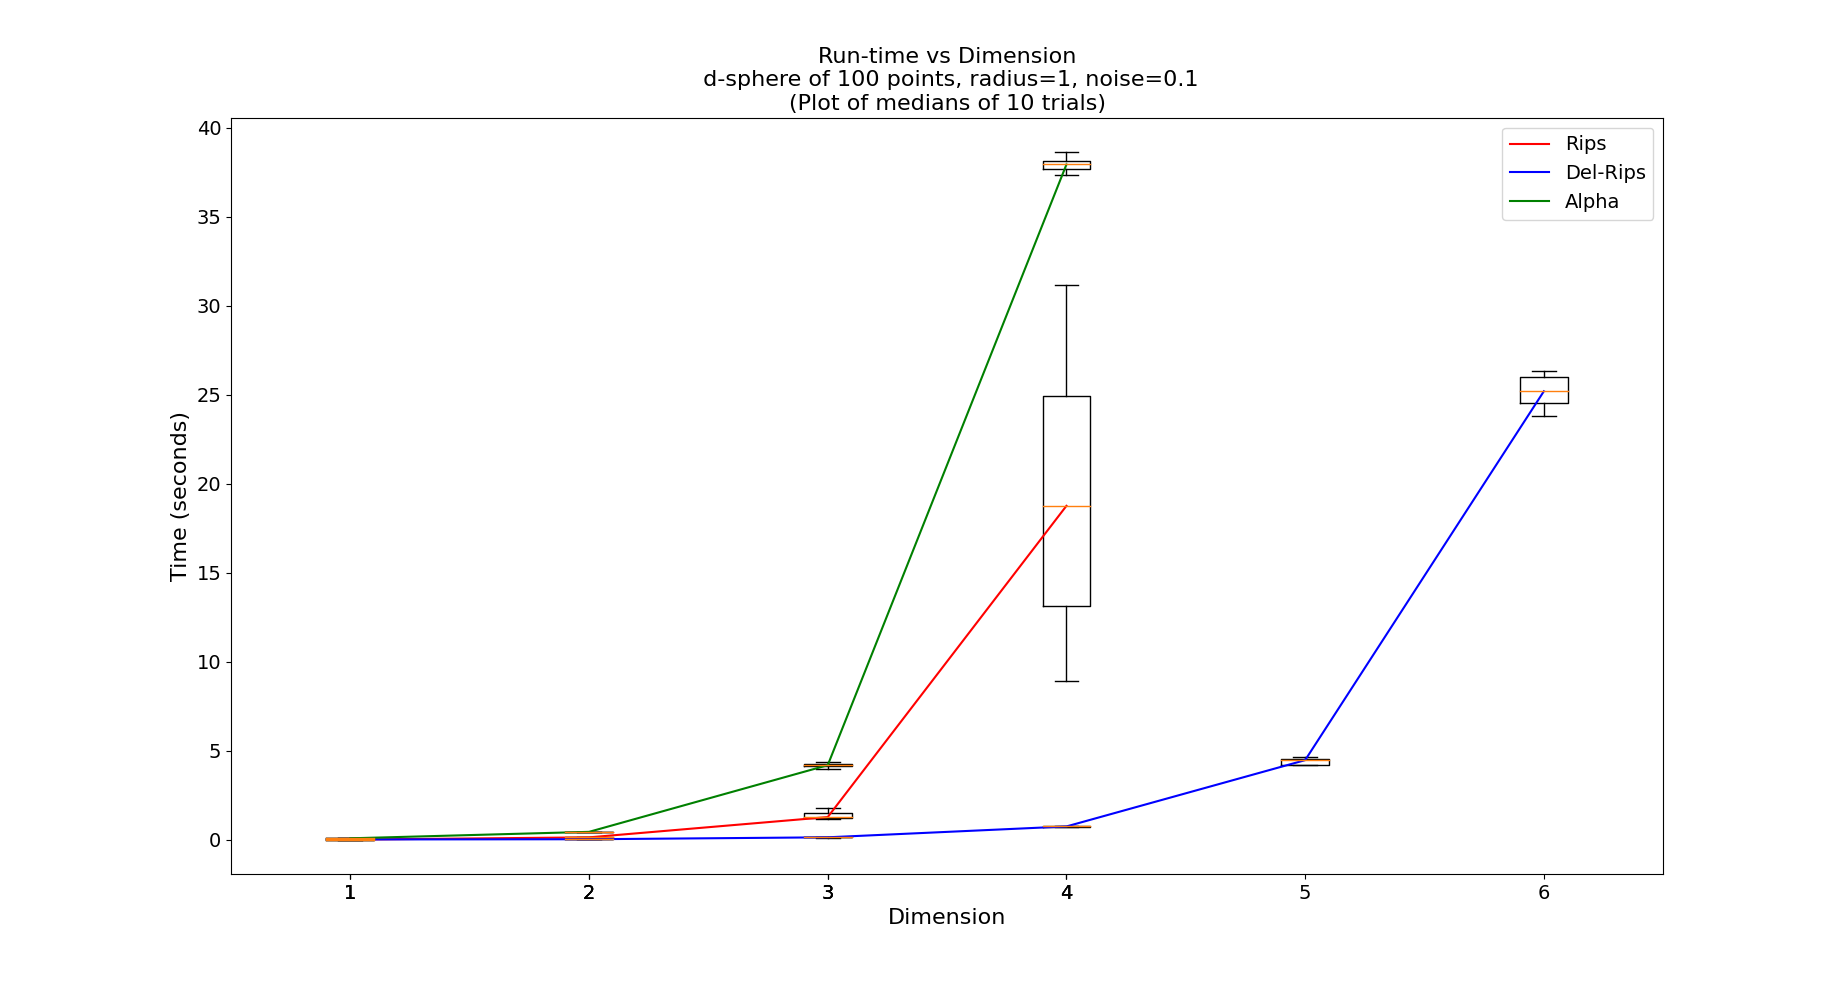
\includegraphics[width=\columnwidth]{./figures/runtime_dim_60sec_cap_1.png}
    \caption{Runtime comparison of Rips, Alpha, and Delaunay-Rips as dimension of data increases.}
    \label{fig:runtime_dim}
\end{figure}



\subsection{Persistence Diagram Instability}
The Delaunay-Rips construction gains computational efficiency at the cost of stability. We demonstrate a simple, yet clear example of how this instability can arise. In figure \ref{fig:4pt_PDs_transformation}, we can visually see a particular configuration of four points giving a radically different Persistence Diagram as we move the right-most point across the circumcircle of the other 3 points. In the figure, we have marked the Delaunay Triangulation of the points to show case the point at which an edge flip occurs (namely when all four points lie on the same circle). We now proceed to formally prove the instability of this particular configuration of points.

\begin{figure}[ht]
    \centering
    \def\svgwidth{\columnwidth}
    \incfig{4pt_PDs_transformation}
    \caption{Persistence Diagrams of 4 point example}
    \label{fig:4pt_PDs_transformation}
\end{figure}

\begin{defn}
    Let $X$ and $Y$ be two non-empty subsets of a metric space $(M,d)$. We define their \textbf{Hausdorff distance} $d_H(X,Y)$ by
    $$d_H(X,Y):=\max\left\{\sup_{x\in X} d(x,Y), \sup_{y\in Y} d(X,y)\right\}.$$
\end{defn}

\begin{defn}
    If $X$ and $Y$ are two compact metric spaces, then the \textbf{Gromov-Haudorff distance} $d_{GH}(X,Y)$ is defined to be the infimum of all numbers $d_H(f(X),g(Y))$ for all metric spaces $M$ and all isometric embeddings $f:X \to M$ and $g:Y \to M$.
\end{defn}

\begin{defn}
    Let $X$ and $Y$ be two persistence diagrams. Let $\eta:X\to Y$ be a bijection and $||x-y||_\infty := \max \{|x_1-y_1|,|x_2-y_2|\}$ for $x=(x_1,x_2), y=(y_1,y_2)$. We define the \textbf{bottleneck distance} between the diagrams as

    $$W_\infty(X,Y) = \inf_{\eta:X\to Y} \sup_{x\in X}||x-\eta(x)||_\infty.$$    
\end{defn}

Let ($\mathcal{P}$, $d_{GH}$) be the space of point clouds equipped with the Gromhov-Hausdorff metric and let ($\mathcal{D}$, $W_\infty$) be the space of Persistence Diagrams equipped with the bottle neck metric. Let
$$Pers_1: \mathcal{P} \to \mathcal{D}$$
where $Pers_1(P)$ is the persistence diagram showing the $H_1$ classes of the point cloud $P$ constructed using the Delaunay-Rips complex. Our example comes from 4 points taken in $\R^2$ where the instability is demonstrated as the discontinuity of $Pers_1$.

Let $P \in \mathcal{P}$ as $P = \{(-1,0),(\frac{1}{2},\frac{\sqrt{3}}{2}),(\frac{1}{2},-\frac{\sqrt{3}}{2}),(1,0)\}.$ Note that the points all lie on the unit circle, so the Delaunay 1-skeleton has an edge between every pair of points (See figure). Thus, $Pers_1(P)$ has no $H_1$ class with non-zero persistence using the Delaunay-Rips filtration, as can be verified by the reader.

Fix $\varepsilon=0.1$. We now show that for any $\delta > 0$, there exists $P' \in \mathcal{P}$ such that $d_{GH}(P,P')< \delta$, but $W_\infty(Pers_1(P), Pers_1(P')) \geq \varepsilon.$ Take $P' = \{(-1,0),(\frac{1}{2},\frac{\sqrt{3}}{2}),(\frac{1}{2},-\frac{\sqrt{3}}{2}),(1-x,0)\}$ with $0<x < \delta < \frac{2-\sqrt{3}}{2}$. This is a small perturbation of $P$ by pushing the point $(1,0)$ inside the unit circle thereby putting the points in general position. We only work with $\delta<2-\sqrt{3}$ so that $Pers_1(P')$ maintains an $H_1$ class with non-zero persistence; for this example to work, we further need $\delta < \frac{2-\sqrt{3}}{2}$. We just compute the Hausdorff distance $d_H$ between $P$ and $P'$ in the plane taking the isometric embedding of $P$ to be the map that sends each of its points to itself in $\R^2$ and the same embedding for $P'$. Since the Gromov-Hausdorff distance is the infimum of $d_H(f(P),g(P'))$ over all isometric embeddings $f:P \to X$ and $g: P' \to X$ into any metric space $X$, $d_H(P,P')$ serves as an upper bound for $d_{GH}(P,P').$ We find that
$$d_{GH}(P,P')\leq d_H(P,P')=x<\delta.$$
Recall that $Pers_1(P)$ has no $H_1$ class with non-zero persistence. Thus, to compute $W_\infty(Pers_1(P),Pers_1(P'))$, we must match the $H_1$ class of $Pers_1(P')$ with the diagonal. The $H_1$ class of $Pers_1(P')$ has birth $\sqrt{3}$ and death $2-x$ as calculated in the Appendix, section \ref{boundary_mat}. Using the max norm, we find
$$d: = W_\infty(Pers_1(P),Pers_1(P')) = 2-x-\sqrt{3} \geq 2-\frac{2-\sqrt{3}}{2} -\sqrt{3} \geq 0.1 = \varepsilon.$$
Hence, our map $Pers_1$ is discontinuous at $P$. This gives us insight into when the Delaunay-Rips construction of the Persistence Diagram experiences instability--namely when points are not in general position. We now have motivation to ask if we have stability of the PD when the underlying Delaunay-Rips complex does not change under a perturbation of the point cloud.


\subsection{Stability in a Neighborhood}\label{stability}
\begin{enumerate}
    \item What is the best our method can do? Use knowledge on stability of Delaunay Triangulation.
\end{enumerate}
    Let $P$ denote our point cloud and $P'$ denote the perturbed point cloud. We use $|xy|$ notation to denote the Euclidean distance between points $x,y \in \R^n$. Let $V_x$ denote the closed Voronoi region for the point $x \in P$. Here is a lemma that should work in $\R^n$:
    \begin{lem}\label{paperlemma}
    Two points $p_i,p_j \in P$ are strong Voronoi neighbors if and only if there exists an $m$ such that
    $$\max\{|mp_i|,|mp_j|\} < \min_{k \neq i,j}|mp_k|.$$
    \end{lem}
    
    We claim
    \begin{thm}
    Let $p_i,p_j \in P$ be strong Voronoi neighbors and $m \in V_{p_i} \cap V_{p_j}$. For $\varepsilon = \min\{\frac{1}{4}(\min_{k \neq i,j}|mp_k|-|mp_j|), \frac{1}{2}\min_{i \neq j} |p_i p_j|\}$, an $\varepsilon$-perturbation of $P$ leaves $p_i$ and $p_j$ as strong Voronoi neighbors.
    \end{thm}
    \begin{proof}
        Let $p_i,p_j \in P$ satisfy Lemma \ref{paperlemma} with $m \in V_{p_i} \cap V_{p_j}$. Note that $0<\varepsilon<\frac{1}{2}\min_{i \neq j} |p_i p_j|$ to ensure a unique correspondence between the points of $P$ and the points of $P'$. We begin with the conclusion of Lemma \ref{paperlemma}:
        $$\max\{|mp_i|,|mp_j|\} < \min_{k \neq i,j}|mp_k|$$
        $$2\max\{|mp_i|,|mp_j|\} < 2\min_{k \neq i,j}|mp_k|$$
        $$\min_{k \neq i,j}|mp_k|+3\max\{|mp_i|,|mp_j|\} < 3\min_{k \neq i,j}|mp_k|+\max\{|mp_i|,|mp_j|\}$$
        $$\frac{1}{4}\min_{k \neq i,j}|mp_k| +\frac{3}{4}\max\{|mp_i|,|mp_j|\} < \frac{3}{4}\min_{k \neq i,j}|mp_k| + \frac{1}{4}\max\{|mp_i|,|mp_j|\}$$
        % $$\max\{|mp_i|,|mp_j|\}+\frac{1}{4}\min_{k \neq i,j}|mp_k|-\frac{1}{4}\max\{|mp_i|,|mp_j|\} < \min_{k \neq i,j}|mp_k| -\frac{1}{4}\min_{k \neq i,j}|mp_k|+\frac{1}{4}\max\{|mp_i|,|mp_j|\}$$
        $$\max\{|mp_i|,|mp_j|\}+\frac{1}{4}(\min_{k \neq i,j}|mp_k|-\max\{|mp_i|,|mp_j|\}) < \min_{k \neq i,j}|mp_k| -\frac{1}{4}(\min_{k \neq i,j}|mp_k|-\max\{|mp_i|,|mp_j|\})$$
        \begin{equation} \label{sandwich_eq}
        \begin{aligned}
            \max\{|mp_i|,|mp_j|\}+\varepsilon \leq \max\{|mp_i|,|mp_j|\}+\frac{1}{4}(\min_{k \neq i,j}|mp_k|-\max\{|mp_i|,|mp_j|\}) \\ < \min_{k \neq i,j}|mp_k| -\frac{1}{4}(\min_{k \neq i,j}|mp_k|-\max\{|mp_i|,|mp_j|\})\leq \min_{k \neq i,j}|mp_k| - \varepsilon.
        \end{aligned}
        \end{equation}
        
        Now, without loss of generality, let
        $$|mp_i'| = \max\{|mp_i'|,|mp_j'|\}.$$
        We note by the triangle inequality that
        \begin{equation}\label{lower_side}
            \max\{|mp_i'|,|mp_j'|\} \leq |mp_i| + |p_ip_i'| \leq \max\{|mp_i|,|mp_j|\} + \varepsilon.
        \end{equation}
        Similarly, we have by the triangle inequality
        \begin{equation}\label{upper_side}
            \min_{k\neq i,j}|mp_k| - \varepsilon = \min_{k\neq i,j}(|mp_k| - \varepsilon) \leq \min_{k\neq i,j}(|mp_k|-|p_kp_k'|) \leq \min_{k \neq i,j} |mp_k'|.
        \end{equation}
        Putting together equations \ref{sandwich_eq}, \ref{lower_side}, \ref{upper_side}, we have
        $$\max\{|mp_i'|,|mp_j'|\} \leq \max\{|mp_i|,|mp_j|\}+\varepsilon < \min_{k \neq i,j}|mp_k| - \varepsilon \leq \min_{k \neq i,j} |mp_k'|.$$
        Thus, we now apply Lemma \ref{paperlemma} and have that $p_i'$ and $p_j'$ remain strong Voronoi neighbors.
    \end{proof}
%%%% Proof with the max and mins written out
    % \begin{proof}
    %     Let $p_i,p_j \in P$ satisfy Lemma \ref{paperlemma} with $m \in V_{p_i} \cap V_{p_j}$. Note that $0<\varepsilon<\frac{1}{2}\min_{i \neq j} |p_i p_j|$ to ensure a unique correspondence between the points of $P$ and the points of $P'$. We define the following to make reading the proof easier
    %     $$|mp| := \max\{|mp_i|,|mp_j|\}$$
    %     $$|mp_k|:= \min_{k \neq i,j}|mp_k|$$
    %     We begin with the conclusion of Lemma \ref{paperlemma}:
    %     $$\max\{|mp_i|,|mp_j|\} < \min_{k \neq i,j}|mp_k|$$
    %     $$2\max\{|mp_i|,|mp_j|\} < 2\min_{k \neq i,j}|mp_k|$$
    %     $$\min_{k \neq i,j}|mp_k|+3\max\{|mp_i|,|mp_j|\} < 3\min_{k \neq i,j}|mp_k|+\max\{|mp_i|,|mp_j|\}$$
    %     $$\frac{1}{4}\min_{k \neq i,j}|mp_k| +\frac{3}{4}\max\{|mp_i|,|mp_j|\} < \frac{3}{4}\min_{k \neq i,j}|mp_k| + \frac{1}{4}\max\{|mp_i|,|mp_j|\}$$
    %     $$\max\{|mp_i|,|mp_j|\}+\frac{1}{4}\min_{k \neq i,j}|mp_k|-\frac{1}{4}\max\{|mp_i|,|mp_j|\} < \min_{k \neq i,j}|mp_k| -\frac{1}{4}\min_{k \neq i,j}|mp_k|+\frac{1}{4}\max\{|mp_i|,|mp_j|\}$$
    %     $$\max\{|mp_i|,|mp_j|\}+\frac{1}{4}(\min_{k \neq i,j}|mp_k|-\max\{|mp_i|,|mp_j|\}) < \min_{k \neq i,j}|mp_k| -\frac{1}{4}(\min_{k \neq i,j}|mp_k|-\max\{|mp_i|,|mp_j|\})$$
    %     \begin{equation} \label{sandwich_eq}
    %         \max\{|mp_i|,|mp_j|\}+\varepsilon \leq \max\{|mp_i|,|mp_j|\}+\frac{1}{4}(\min_{k \neq i,j}|mp_k|-\max\{|mp_i|,|mp_j|\}) < \min_{k \neq i,j}|mp_k| -\frac{1}{4}(\min_{k \neq i,j}|mp_k|-\max\{|mp_i|,|mp_j|\})\leq \min_{k \neq i,j}|mp_k| - \varepsilon.
    %     \end{equation}
    %     Now, without loss of generality, let
    %     $$|mp_i'| = \max\{|mp_i'|,|mp_j'|\}.$$
    %     We note by the triangle inequality that
    %     \begin{equation}\label{lower_side}
    %         \max\{|mp_i'|,|mp_j'|\} \leq |mp_i| + |p_ip_i'| \leq \max\{|mp_i|,|mp_j|\} + \varepsilon.
    %     \end{equation}
    %     Similarly, we have by the triangle inequality
    %     \begin{equation}\label{upper_side}
    %         \min_{k\neq i,j}|mp_k| - \varepsilon = \min_{k\neq i,j}|mp_k - \varepsilon| \leq \min_{k\neq i,j}(|mp_k|-|p_kp_k'|) \leq \min_{k \neq i,j} |mp_k'|.
    %     \end{equation}
    %     Putting together equations \ref{sandwich_eq}, \ref{lower_side}, \ref{upper_side}, we have the theorem as desired.
    %     $$\max\{|mp_i'|,|mp_j'|\} \leq \max\{|mp_i|,|mp_j|\}+\varepsilon < |mp_k| - \varepsilon \leq \min_{k \neq i,j} |mp_k'|.$$
    % \end{proof}

    % \textbf{Alternate attempt at proof:}
    % \newline
    % To keep things simple, we work with our point cloud $P \subset \R^2$ with the idea being
    % \begin{enumerate}
    %     \item Assume that the points of $P$ are in general position and affinely independent
    %     \begin{enumerate}
    %         \item No 4 points lie on the same circle
    %         \item No 3 points lie on the same line
    %     \end{enumerate}
    %     \item Look at 3 points, $p_1, p_2, p_3 \in P$ and find the circumcircle, $C_{p_1p_2p_3}$ through them.
    %     \begin{enumerate}
    %         \item This circle must have a finite radius and finite circumcenter by assumption of affine independence
    %     \end{enumerate}
    %     \item Embark on a mission to find $\varepsilon$ around each point in $P$ such that an $\varepsilon$-perturbation of $P$, call it $P'$, ensures all other points $p_k' \in P'$ stayed inside $C_{p_1'p_2'p_3'}$ if $p_k \in P$ was inside $C_{p_1p_2p_3}$ to begin with or stayed outside if $p_k \in P$ was outside of $C_{p_1p_2p_3}$ to begin with.
    %     \begin{enumerate}
    %         \item We must ensure that there is an $\varepsilon$ so that the points in $P'$ are affinely independent--this ensures that moving the points of $P$ within the $\varepsilon$ balls around each point of $P$ only cause continuous changes in membership of $p_k$ relative to $C_{p_1p_2p_3}$.
    %         \begin{enumerate}\label{colin}
    %             \item Let $O_1 \in \R^2$ denote the circumcenter of the circle $C_{p_1p_2p_3}$. Since the points of $P$ are affinely independent, $O_1$ is not infinite in any of its coordinates. We can specifically calculate $O_1$ by finding the intersection of the perpendicular bisectors of $\overline{p_1p_2}$ and $\overline{p_1p_3}$. We proceed by linear algebra. The process is
    %             \begin{enumerate}
    %                 \item Find midpoint of line segment ($\mathbf{r_0}$)
    %                 \item Find directional vector based at the midpoint that points at one of the ends of the line segments (this acts as the normal vector $\mathbf{n}$ to the perpendicular bisector)
    %                 \item Find the equation of the perpendicular bisector using
    %                 $$\mathbf{n}\cdot \mathbf{r}=\mathbf{n} \cdot \mathbf{r_0}.$$
    %             \end{enumerate}
    %             Once the equations of all necessary perpendicular bisectors are found, we can easily check if they have a solution by checking the determinant of the $2\times 2$ matrix
    %             $$\begin{pmatrix}
    %                 \mathbf{n}_{p_1p_2} & \mathbf{n}_{p_1p_3}
    %             \end{pmatrix}$$
    %             Since the normal vectors are just the directional vectors based at the midpoint pointing towards one of the ends of the line segments, we have that
    %             $$\mathbf{n}_{p_ip_j} = p_j - \frac{p_j-p_i}{2} = \frac{p_j-p_i}{2}.$$
    %             Coming back to our example of $C_{p_1p_2p_3}$ and letting $p_i = (p_{i1},p_{i2})$, we now construct the following sequence of maps:
    %             $$\R^2\times \R^2 \times \R^2 \overset{f}\to \mathcal{M}_{2\times 2}(\R) \cong \R^4 \overset{\det}\to \R$$
    %             where 
    %             $$f(p_1,p_2,p_3):=((p_{21}-p_{11})/2,(p_{22}-p_{12})/2,(p_{31}-p_{11})/2,(p_{32}-p_{12})/2)$$
    %             and $\det$ is the standard determinant function. Let $A=((p_{21}-p_{11})/2,(p_{22}-p_{12})/2,(p_{31}-p_{11})/2,(p_{32}-p_{12})/2)$. Since the determinant is a continuous map, we have that for $\varepsilon = \det(A)/2$, there exists a $\delta_1$ around $A$ such that $\det(A) < \varepsilon$ when $||A|| < \delta_1$. Since $f$ is continuous in each of it's components, $f$ itself is continuous. Thus, there exists $\delta_2$ around each $p_1,p_2,p_3$ such that $||f(p_1,p_2,p_3)||=||A|| < \delta_1$ whenever $|p_i| < \delta_2$.
    %             \newline
    %             To summarize, we have found a neighborhood $\delta_2$ around each point $p_1,p_2,p_3$ that ensures that determinant of the matrix of coefficients of the equation of the perpendicular bisectors is non-zero. This guarantees the three points do not become colinear.
    %         \end{enumerate}
    %         \item We must ensure that there is an $\varepsilon$ so that the points in $P'$ are in general position--this ensures that no $p_k$ change membership relative to $C_{p_1p_2p_3}$.
    %         \begin{enumerate}
    %             \item We have to find this $\varepsilon$ to be less that $\delta_2$. This ensures moving the points of $P$ in the $\varepsilon$-neighborhood around each point changes the radius and circumcenter of $C_{p_1p_2p_3}$ continuously. Since all other $p_k \in P$ change continuously into $p_k' \in P'$, we must have that the smallest distance between $C_{p_1p_2p_3}$ and each $p_k \in P$ for $k \neq 1,2,3$ changes continuously. Thus, if $p_k$ is outside of $C_{p_1p_2p_3}$, then it must lie on the circle $C_{p_1p_2p_3}$ before changing membership into the inside. In other words, we need to find $\varepsilon$ so that $p_1,p_2,p_3,p_k$ do not become cocircular. One way to do this is to ensure the circles $C_{p_1p_2p_3}$ and $C_{p_kp_2p_3}$ do not coincide (do not have the same radius and circumcenter).
    %             \item Let $O_k$ be the circumcenter of the circle $C_{p_kp_2p_3}$ and $O_1$ the circumcenter of $C_{p_1p_2p_3}$. Using a similar argument with a similar of sequence of maps from \ref{colin}, we can find $\delta_3$ around $p_1, p_2, p_3, p_k$ that make sure $O_1 \neq O_k$.
    %             \item My claim 1: $O_1$ and $O_k$ lie on the perpendicular line to the simplex $p_2p_3$ that also goes through the circumcenter of the circle $C_{p_2p_3}$, call it $O_{23}$ (in $\R^2$, this circumcenter is the midpoint of $p_2$ and $p_3$.)
    %             \item My claim 2: $p_k$ on $C_{p_kp_2p_3}$ changes membership relative to $C_{p_1p_2p_3}$ if $O_k$ moves to the other side of $O_1$ along the line going through $O_1$ and $O_{23}$. Thus, since $O_1$ never equals $O_k$ for our chosen $\delta_3$ and $O_1$ and $O_k$ move continuously, we have that $p_k$ remains outside (or inside) the circle $C_{p_1p_2p_3}$.
    %         \end{enumerate}
    %         % \begin{enumerate}
    %         %     \item Let $C_{p_kp_2p_3}$ denote the circle through $p_k, p_2, p_3$ for some $k \neq 1,2,3$. Let $O_1 \in R^2$ denote the circumcenter of the circle $C_{p_1p_2p_3}$ and $O_k \in R^2$ denote the circumcenter of $C_{p_k,p_2,p_3}$. Since the points of $P$ are in general position, $O_1 \neq O_k.$ Thus
    %         %     $$d(O_1,O_k) > 0.$$ 
    %     \end{enumerate}
    %     \item Repeat this for $n$ choose $3$ points and find the $\varepsilon$s associated with each circle formed by them to keep points from changing membership relative to them. Take the final $\varepsilon$ to be the minimum of all of these $\varepsilon$s. This ensures that $P'$ has the same Delaunay triangulation as $P$.
    % \end{enumerate}
    
    \begin{lem}\label{affine_indep_lemma}
        Given a subset $S= \{p_1,p_2,\dots,p_{d+1}\} \subset P$, there exists $\varepsilon>0$ such that any $\varepsilon$-perturbation $S'$ of $S$ has $\{p_1',p_2',\dots,p_{d+1}'\} \subset P'$ as linearly independent.
    \end{lem}
    \begin{proof}
        Let $\Sph$ be the unique $(d-1)$-sphere containing $S$ with center $O$. We proceed by linear algebra, treating each $p_i$ as a vector $\mathbf{p_i} \in \R^d$. We locate the center $O \in \R^d$ by finding the intersection of the perpendicular bisecting planes to the line segments $\overline{\mathbf{p_2}\mathbf{p_1}}, \overline{\mathbf{p_3}\mathbf{p_1}}, \dots, \overline{\mathbf{p_{d+1}}\mathbf{p_1}}$.
        % Check why any d hyperplanes made using pairs of the points S define the same circumcenter
        Thus, we will have $d$ hyperplanes each in $d$ variables: this is a system of linear equations that has a solution since our subset $S$ is in general position (that is, no two perpendicular bisecting hyperplanes are parallel). The vector equation for the perpendicular bisecting hyperplane of $\overline{\mathbf{p_i}\mathbf{p_1}}$ can be found by determining the normal vector and a point on the hyperplane. A point on the plane we can use is simply the midpoint of $\overline{\mathbf{p_i}\mathbf{p_1}}$:
        $$\mathbf{b_i} := \frac{\mathbf{p_i}+\mathbf{p_1}}{2}.$$
        The normal vector to the plane is the directional vector based at the midpoint and pointing in the direction of one end of the line segment $\overline{\mathbf{p_i}\mathbf{p_1}}$. We find the normal vector to be
        $$\mathbf{n_i} := \mathbf{p_i}-\mathbf{b_i} = \frac{\mathbf{p_i}-\mathbf{p_1}}{2}.$$
        Thus, the vector equation of the perpendicular bisecting hyperplane of $\overline{\mathbf{p_i}\mathbf{p_1}}$ is
        $$\mathbf{n_i}\cdot \mathbf{r}=\mathbf{n_i}\cdot\mathbf{b_i}$$
        where $\mathbf{r}$ is the position vector for an arbitrary point on the hyperplane.
        \newline
        We are now ready to construct the following maps whose composition will output the circumcenter $O \in \R^d$ as a function of the $d+1$ points defining the sphere $\Sph$. We illustrate an example of this with 3 points in $\R^2$ in figure \ref{fig:circumcenter}. This construction is instrumental to obtaining $\varepsilon$ balls around each point that ensures the circumcenter $O$ remains bounded. Define

        $$f:\underbrace{\R^d \times \dots \times \R^d}_{d+1} \to \mathcal{M}_{d}(\R)\times \R^d$$
        $$f:(\mathbf{p_1},\mathbf{p_2},\dots,\mathbf{p_{d+1}}) \mapsto \left(\begin{bmatrix}
            \mathbf{n_2}\\ \mathbf{n_3}\\ \vdots\\ \mathbf{n_{d+1}}
        \end{bmatrix},
        \begin{bmatrix}
            \mathbf{n_2}\cdot\mathbf{b_2} \\ \mathbf{n_3}\cdot\mathbf{b_3}\\ \vdots \\ \mathbf{n_{d+1}}\cdot\mathbf{b_{d+1}}
        \end{bmatrix}\right)$$
        $$g:\text{GL}_d(\R)\times \R^d \to \R^d$$
       
            
        $$g:(A,b) \mapsto A\inv b.$$
        \begin{figure}[ht]
            \centering
            \def\svgwidth{.7\textwidth}
            \incfig{circumcenter}
            \caption{Locating the circumcenter of 3 points in $\R^2$ as a function of the 3 points.}
            \label{fig:circumcenter}
        \end{figure}
        We prove that the map $f$ is continuous. Let the domain of $f$ have the the standard topology of $\R^{d(d+1)}$ (i.e. the open balls in $\R^{d(d+1)}$ form a basis for the topology). Observing that $\mathcal{M}_{d} \cong \R^{d^2}$, we have $\mathcal{M}_{d}(\R)\times \R^d \cong \R^{d^2}\times \R^d \cong \R^{d(d+1)}$. We let this space have the standard topology of $\R^{d(d+1)}$. Note that $f$ is a polynomial in each component of it's output by how it is defined. Thus, $f$ itself is continuous.

        We carefully prove that the map $g$ is continuous. Let $\R^d$ have the standard topology and $\text{GL}_d(\R)\times \R^d$ have the subspace topology of $\mathcal{M}_{d}(\R)\times \R^d$. Note that taking the inverse of a matrix is a continuous function in the topology induced by the Frobenius norm (proven in detail in Section \ref{continuity_of_inverse}). Mapping $b \mapsto b$ is a continuous function in the standard topology of $\R^d$. Since these two functions are defined on spaces with the same topology, recall that the product of two continous functions is continuous. Hence, $g(A,b)=A\inv b$ is a continuous function.
        % reference why A\inv and multiplication of vectors is continuous.
        
        Observe that $g \circ f$ is the circumcenter of the sphere through the input points. This composition is continous since $g$ and $f$ are continous. Let $p = (\mathbf{p_1},\mathbf{p_2},\dots,\mathbf{p_{d+1}}) \in \R^{d(d+1)}$ and let $O=g \circ f(p)$. Thus, for any $\varepsilon_1>0$, there exists a $\delta>0$ such that when $p'=(\mathbf{p_1}',\mathbf{p_2}',\dots,\mathbf{p_{d+1}}')$ satisfies $||p-p'|| < \delta$, then
        $$||O-O'|| < \varepsilon_1$$
        where $O'=g \circ f(p').$ Thus, we have that $B_\delta(p) \subset \R^{d(d+1)}$ is an open ball of radius $\delta$ centered at $p$. Let $\pi_i$ be the projection map that projects $p$ into its $i$th coordinate:
        $$\pi_i: \underbrace{\R^d \times \dots \times \R^d}_{d+1} \to \R^d$$
        $$\pi_i: (\mathbf{p_1},\mathbf{p_2},\dots,\mathbf{p_{d+1}}) \mapsto \mathbf{p_i}.$$
        This map is an open map, thus $\pi_i(B_\delta(p))$ is an open set in $\R^d$. Since we have $\mathbf{p_i} \in \pi_i(B_\delta(p))$ by definition, we can find an open ball $B_{\delta_i}(\mathbf{p_i}) \subset \R^d$ for each $1\leq i \leq d+1$. Letting $\varepsilon = \min\{\delta_i\}_{i=1}^{d+1}$, we have an $\varepsilon$ neighborhood around each point $\mathbf{p_i}$ defining $\mathcal{S}$ that ensures the circumcenter $O$ stays in an $\varepsilon_1$ ball.

        % $$\underbrace{\R^d \times \dots \times \R^d}_{d+1} \xrightarrow{f} \mathcal{M}_{d\times d}\times \R^d \xrightarrow{g} \R^d$$
        % $$f:(p_1,p_2,\dots,p_{d+1}) \mapsto \left(\frac{\mathbf{p_2}-\mathbf{p_1}}{2}\ \frac{\mathbf{p_3}-\mathbf{p_1}}{2}\dots \frac{\mathbf{p_{d+1}}-\mathbf{p_1}}{2}\right),\left(\left|\frac{\mathbf{p_2}+\mathbf{p_1}}{2}\right|^2, \left|\frac{\mathbf{p_3}+\mathbf{p_1}}{2}\right|^2,\dots,\left|\frac{\mathbf{p_{d+1}}-\mathbf{p_1}}{2}\right|^2\right)$$
        % $$g:(A,b) \mapsto \frac{1}{\det(A)}adj(A^T)b$$
    \end{proof}
    
\begin{lem}\label{stay-delaunay}
        For a Delaunay simplex $D= \{p_1,p_2,\dots,p_{d+1}\} \subset P$, there exists $\varepsilon>0$ such that any $\varepsilon$-perturbation $D'$ of $D$ has $\{p_1',p_2',\dots,p_{d+1}'\} \subset P'$ as a Delaunay simplex.
    \end{lem}
    \begin{proof}
        Let $\Sph$ be the unique $(d-1)$-sphere containing $D$ with center $O$. Since $D$ is a Delaunay simplex, for all $p_k \in P\backslash D$, $d(O,p_1) < d(O,p_k$). Let $t(p_k):=(d(O,p_k)-d(O,p_1))/4$ and select $p_{\min} \in P\backslash{D}$ that minimizes $t$. It follows that,
        $$d(O,p_1)+2t=d(O,p_{\min})-2t.$$
        Since $P$ is in general position and finite, $t>0$. Let $\varepsilon_1 = t$, then we obtain from Lemma \ref{affine_indep_lemma} that there is $\delta>0$ such that each $d(p_i,p_i')<\delta$ for $i=1,2,\dots,d+1$ implies $d(O,O')<\varepsilon_1$. Now, we take $\varepsilon = \min(\delta, \varepsilon_1)$ and $D'$ is the $\varepsilon$-perturbation of $D$. Let $\Sph'$ be the unique $(d-1)$-sphere containing $D'$ with center $O'$. Using the triangle inequality, we have the following chains of inequalities:
        $$d(O',p_1') \leq d(O',O)+d(O,p_1)+d(p_1,p_1')$$
        $$< \varepsilon_1 + d(O,p_1)+\delta \leq t+d(O,p_1)+t$$
        $$= d(O,p_1)+2t = d(O,p_{\min})-2t.$$
        Since $d(O,p_{\min})$ minimized $t$, it must be that $d(O,p_{\min}) \leq d(O,p_k)$ for any $p_k \in P\backslash D$. Thus, we have
        $$d(O,p_{\min})-2t \leq d(O,p_k)-t-t < d(O,p_{k})-\varepsilon_1-\delta$$
        $$\leq d(O,p_{k})-d(O,O')-d(p_{k},p_{k}') \leq d(O',p_{k}').$$
        We have concluded that
        $$d(O',p_1')<d(O',p_{k}')$$
        for any $p_k' \in P'\backslash D'$. Hence, $D'$ is a Delaunay simplex.
    \end{proof}
    % \begin{proof} My proof with t/8
    %     Let $\Sph$ be the unique $(d-1)$-sphere containing $D$ with center $O$. Since $D$ is a Delaunay simplex, for all $p_k \in P\backslash D$, $d(O,p_1) < d(O,p_k$). Let $t(p_k):=d(O,p_k)-d(O,p_1)$ and select $p_{\min} \in P\backslash{D}$ that minimizes $t$. Since $P$ is in general position and finite, $t>0$. Let $\varepsilon_1 = t/8$, then we obtain from Lemma \ref{affine_indep_lemma} that there is $\delta>0$ such that each $d(p_i,p_i')<\delta$ for $i=1,2,\dots,d+1$ implies $d(O,O')<\varepsilon_1$. Now, we take $\varepsilon = \min(\delta, \varepsilon_1)$ and $D'$ is the $\varepsilon$-perturbation of $D$. Let $\Sph'$ be the unique $(d-1)$-sphere containing $D'$ with center $O'$. Using the triangle inequality, we have the following chains of inequalities:
    %     $$d(O',p_1') \leq d(O',O)+d(O,p_1)+d(p_1,p_1') \leq \varepsilon_1 + d(O,p_1)+\delta \leq \frac{t}{8}+d(O,p_1)+\frac{t}{8}=d(O,p_1)+\frac{1}{4}t$$
    %     $$< d(O,p_1)+\frac{3}{4}t = d(O,p_1)+t-\frac{1}{4}t = d(O,p_{\min})-\frac{1}{4}t \leq d(O,p_k)-\frac{1}{4}=d(O,p_{k})-\frac{t}{8}-\frac{t}{8}$$
    %     $$\leq d(O,p_{k})-\varepsilon_1-\delta \leq d(O,p_{k})-d(O,O')-d(p_{k},p_{k}') \leq d(O',p_{k}').$$
    %     This inequality is true for any $p_k' \in P'\backslash D'$. Hence, $D'$ is a Delaunay simplex.
    % \end{proof}

    \begin{lem}\label{stay-non-delaunay}
        For a non-Delaunay simplex $D= \{p_1,p_2,\dots,p_{d+1}\} \subset P$, there exists $\varepsilon>0$ such that any $\varepsilon$-perturbation $D'$ of $D$ has $\{p_1',p_2',\dots,p_{d+1}'\} \subset P'$ as a non-Delaunay simplex.
    \end{lem}
    \begin{proof}
        An illustrated example can be found in figure \ref{fig:non-delaunay}. Let $\Sph$ be the unique $(d-1)$-sphere containing $D$ with center $O$. Since $D$ is a non-Delaunay simplex, there exists a $p_k \in P\backslash D$ such that $d(O,p_k) < d(O,p_1)$. Let $t:=(d(O,p_1)-d(O,p_k))/4$ so that 
        $$d(O,p_k)+2t = d(O,p_1)-2t.$$
        Since $P$ is in general position, $t > 0$. Let $\varepsilon_1 = t$, then we obtain from Lemma \ref{affine_indep_lemma} that there is $\delta>0$ such that each $d(p_i,p_i')<\delta$ for $i=1,2,\dots,d+1$ implies $d(O,O')<\varepsilon_1$. Now, we take $\varepsilon = \min(\delta, \varepsilon_1)$ and $D'$ is the $\varepsilon$-perturbation of $D$. Let $\Sph'$ be the unique $(d-1)$-sphere containing $D'$ with center $O'$. Using the triangle inequality, we have the following chains of inequalities:
        $$d(O',p_k') \leq d(O',O)+d(O,p_k)+d(p_k,p_k') $$
        $$< \varepsilon_1 + d(O,p_k)+\delta \leq t+d(O,p_k)+t$$
        $$=d(O,p_k)+2t= d(O,p_1)-2t$$
        $$=d(O,p_1)-t-t \leq d(O,p_1)-\varepsilon_1-\delta$$
        $$< d(O,p_1)-d(O,O')-d(p_1,p_1') \leq d(O',p_1').$$
        Since $d(O',p_1')$ is the radius of $\Sph'$, we have that $p_k' \in \interior(\Sph')$. Hence, $D'$ is a non-Delaunay simplex.
    \end{proof}
    
    \begin{figure}[ht!]
        \centering
        \def\svgwidth{0.6\columnwidth}
        \incfig{non-delaunay}
        \caption{Maintaing a non-Delaunay triangle in $\R^2$. We take $\varepsilon = \min(\delta,\varepsilon_1)$. We illustrate in this figure how $p_k'$ remains within the circumcircle through $p_1', p_2',$ and $p_3'$.}
        \label{fig:non-delaunay}
    \end{figure}

    % \begin{proof} My t/8 argument
    %     Let $\Sph$ be the unique $(d-1)$-sphere containing $D$ with center $O$. Since $D$ is a non-Delaunay simplex, there exists a $p_k \in P\backslash D$ such that $d(O,p_k) < d(O,p_1)$. Let $t:=d(O,p_1)-d(O,p_k)$. Since $P$ is in general position, $t>0$. Let $\varepsilon_1 = t/8$, then we obtain from Lemma \ref{affine_indep_lemma} that there is $\delta>0$ such that each $d(p_i,p_i')<\delta$ for $i=1,2,\dots,d+1$ implies $d(O,O')<\varepsilon_1$. Now, we take $\varepsilon = \min(\delta, \varepsilon_1)$ and $D'$ is the $\varepsilon$-perturbation of $D$. Let $\Sph'$ be the unique $(d-1)$-sphere containing $D'$ with center $O'$. Using the triangle inequality, we have the following chains of inequalities:
    %     $$d(O',p_k') \leq d(O',O)+d(O,p_k)+d(p_k,p_k') \leq \varepsilon_1 + d(O,p_k)+\delta \leq \frac{t}{8}+d(O,p_k)+\frac{t}{8}=d(O,p_k)+\frac{1}{4}t$$
    %     $$< d(O,p_k)+\frac{3}{4}t = d(O,p_k)+t-\frac{1}{4}t = d(O,p_1)-\frac{1}{4}t = d(O,p_1)-\frac{t}{8}-\frac{t}{8}$$
    %     $$\leq d(O,p_1)-\varepsilon_1-\delta \leq d(O,p_1)-d(O,O')-d(p_1,p_1') \leq d(O',p_1').$$
    %     Since $d(O',p_1')$ is the radius of $\Sph'$, we have that $p_k' \in \interior(\Sph')$. Hence, $D'$ is a non-Delaunay simplex.
    % \end{proof}
    
    
    \begin{thm}
        Let $P \subset \R^d$ be in general position, that is no $d+2$ points lie on the same $(d-1)$-sphere and no $d+1$ points are affinely dependent. Then, there exists $\varepsilon>0$ such that any $\varepsilon$-perturbation $P'$ of $P$ has the same Delaunay Triangulation as $P$. That is,
        $$\Del(P) = \Del(P').$$
    \end{thm}
    \begin{proof}
        Let $D$ be a subset of $P$ of size $d+1$. Depending if $D$ is a Delaunay simplex in $P$, obtain $\varepsilon_D$ from Lemma \ref{stay-delaunay} or from Lemma \ref{stay-non-delaunay}. For any $\varepsilon_D$-perturbation $D'$ of $D$, we have $Del(D)=Del(D')$. Now, find
        $$\varepsilon = \min \{\varepsilon_D\ |\ \text{for every}\ D \subset P\}.$$
        Hence, for any $\varepsilon$-perturbation $P'$ of $P$, $P'$ has the same Delaunay Triangulation as $P$.
    \end{proof}
    
    Now, we need a theorem that gives us stability of PDs in PD space equipped with the bottle-neck distance. So,



    
\section{Application of Delaunay-Rips}
\begin{enumerate}
    \item Demonstrate value by talking about as dimensions change and number of points change.
    \item Particular examples of how using special data sets affect the run-time of Rips/Alpha drastically but maybe not Del-Rips.
    \item Performance: accuracy in ML algorithm, or classification. Instability may cause performance to go down even though run-time is unaffected.
\end{enumerate}

\subsection{Synthetic Data}
    Focus is two things: Accuracy and Speed. Demonstrating accuracy (by comparing with Rips and Alpha) builds trust in Del-Rips. Demonstrating speed encourages using Del-Rips over Rips or Alpha.

    Comparing Ripser, Cechmate's Alpha, and our Del-Rips implementation.
    \begin{enumerate}
        \item Data 1: Noisy 1000 pt 1-sphere
        \item Data 2: Noisy 100 pt. 2-sphere
        \item Data 3: Noisy 100 pt. Torus in 3 dimensions
        \item Data 4: Noisy 100 pt. Klein bottle in 4 dimensions
    \end{enumerate}

    Section with tables. Make a table with a column labeled ``Rips" and the other column labeled ``Alpha". Each row of the table is a data set. In each cell of the table, put the PD for the corresponding column method alongside the PD made by using Del-Rips. Place underneath the bottleneck distance between the two PDs. Do this for each data set (row).

    Next table will have 3 columns (Rips, Alpha, Del-Rips). Each row is (again) a data set. Each cell will be the corresponding run-time (in seconds).
       
    \textbf{Need a better measurement of accuracy: maybe look at a classification problem (see how the quality of prediction is affected when using del-rips)}

    Section with graphs. First graph will be of a 2-sphere with points increasing from 100-10,000 with runtime on the y-axis. Second graph will be a $d$-sphere of 50 points with dimension increasing from 2-7 with the runtime on the y-axis. Each graph will compare Rips, Alpha, and Del-Rips.
    \textbf{plot the standard deviation along each curve for each data point: or better, a box-whisker plot at each point for this non-gaussian distribution}
    
    Note that we are comparing runtime of packages, not the run time of the filtration. So the theoretical runtime analysis will not compare with the actual runtime in this section. Or, we could compare rips (cechmate), alpha (cechmate), del-rips because they all use PHAT to reduce the boundary matrix and then the only comparison to make would be the filtration step.
    
    Highlight separately the speed up in the filtration step and then the PD step (since you have less simplices).


\subsection{Real Data}



\section{Conclusion}



\subsection{Further Questions}


\appendix
\section{Appendix: Math}

\subsection{Boundary Matrix Calculation for Instability}\label{boundary_mat}

\begin{figure}[ht]
    \centering
    \def\svgwidth{\columnwidth}
    \incfig{4pt_filtration}
    \caption{filtration}
    \label{fig:4pt_filtration}
\end{figure}

We have $P' = \{(-1,0),(\frac{1}{2},\frac{\sqrt{3}}{2}),(\frac{1}{2},-\frac{\sqrt{3}}{2}),(1-x,0)\}$ with $0< x < \delta < 2-\sqrt{3}$.
Our filtration has 4 key scale values, $t = 0<\sqrt{1-x+x^2}< \sqrt{3}< 2-\delta$ as shown in Figure \ref{fig:4pt_filtration}. We construct our boundary matrix $B$ and reduce it to $\overline{B}$ using the standard algorithm:
$$B=\bordermatrix{ 
    &   a & b & c & d & bd & cd & ab & ac & ad & abd & acd\cr
    a & 0 & 0 & 0 & 0 &  0 &  0 &  1 &  1 &  1 &   0 &   0 \cr
    b & 0 & 0 & 0 & 0 &  1 &  0 &  1 &  0 &  0 &   0 &   0\cr
    c & 0 & 0 & 0 & 0 &  0 &  1 &  0 &  1 &  0 &   0 &   0\cr
    d & 0 & 0 & 0 & 0 &  1 &  1 &  0 &  0 &  1 &   0 &   0\cr
   bd & 0 & 0 & 0 & 0 &  0 &  0 &  0 &  0 &  0 &   1 &   0\cr
   cd & 0 & 0 & 0 & 0 &  0 &  0 &  0 &  0 &  0 &   0 &   1\cr
   ab & 0 & 0 & 0 & 0 &  0 &  0 &  0 &  0 &  0 &   1 &   0\cr
   ac & 0 & 0 & 0 & 0 &  0 &  0 &  0 &  0 &  0 &   0 &   1\cr
   ad & 0 & 0 & 0 & 0 &  0 &  0 &  0 &  0 &  0 &   1 &   1\cr
  abd & 0 & 0 & 0 & 0 &  0 &  0 &  0 &  0 &  0 &   0 &   0\cr
  acd & 0 & 0 & 0 & 0 &  0 &  0 &  0 &  0 &  0 &   0 &   0\cr
    } \qquad$$
$$\overline{B}=\bordermatrix{ 
    &   a & b & c & d & bd & cd & ab & ac & ad & abd & acd\cr
    a & 0 & 0 & 0 & 0 &  0 &  0 &  1 &  0 &  0 &   0 &   0 \cr
    b & 0 & 0 & 0 & 0 &  1 &  1 &  1 &  0 &  0 &   0 &   0\cr
    c & 0 & 0 & 0 & 0 &  0 &  1 &  0 &  0 &  0 &   0 &   0\cr
    d & 0 & 0 & 0 & 0 &  1 &  0 &  0 &  0 &  0 &   0 &   0\cr
   bd & 0 & 0 & 0 & 0 &  0 &  0 &  0 &  0 &  0 &   1 &   1\cr
   cd & 0 & 0 & 0 & 0 &  0 &  0 &  0 &  0 &  0 &   0 &   1\cr
   ab & 0 & 0 & 0 & 0 &  0 &  0 &  0 &  0 &  0 &   1 &   1\cr
   ac & 0 & 0 & 0 & 0 &  0 &  0 &  0 &  0 &  0 &   0 &   1\cr
   ad & 0 & 0 & 0 & 0 &  0 &  0 &  0 &  0 &  0 &   1 &   0\cr
  abd & 0 & 0 & 0 & 0 &  0 &  0 &  0 &  0 &  0 &   0 &   0\cr
  acd & 0 & 0 & 0 & 0 &  0 &  0 &  0 &  0 &  0 &   0 &   0\cr
    }. \qquad$$
The persistence pairs for the $H_0$ class with their persistence diagram coordinate (birth/death pair) come out as follows:
$$(a,N/A): (0,\infty)$$
$$(b,ab): (0,\sqrt{3})$$
$$(c, cd): (0,\sqrt{1-x+x^2})$$
$$(d, bd): (0,\sqrt{1-x+x^2}).$$
The $H_1$ classes come out as
$$(ad, abd): (2-x, 2-x)$$
$$(ac, acd): (\sqrt{3}, 2-x).$$
The only point with non-zero persistence is $(\sqrt{3}, 2-x).$


\subsection{Continuity of Matrix Inverse} \label{continuity_of_inverse} %should I make V=GL_n?
Let $V=(\mathcal{M}_n(\R), ||\cdot||)$ be the normed vector space of $n\times n$ matrices over $\R$ with the Frobenius norm defined as
$$||A||_F = \sqrt{\sum_{i=1}^n\sum_{j=1}^na_{ij}^2}$$
where $a_{ij}$ is the entry in the $i$th row and $j$th column of $A$. Recall the definition of the vector 2-norm
$$||v||_2 = \sqrt{\sum_{i=1}^n |v_i|^2}$$
for $v \in \R^n$. We use the vector 2-norm with the Frobenius matrix norm because of their compatibility: that is, 
$$||Mv||_2 \leq||M||_F||v||_2.$$
We proceed by dropping the subscripts and using $||\cdot||$ for matrix and vector norms.

The heavy machinery used to establish the continuity of the matrix inverse was done in \cite{Wilkinson} pages 92-93. However, their proof did not explicitly compute inequalities involving the Frobenius norm (that is, $||I|| = \sqrt{n}$ for $I \in V$ being the identity). For completeness, we provide derivations of similar results using the Frobenius norm.

\begin{lem}\label{lem:AplusE_invertible}
    Given $A,E \in V$ with $A$ invertible, the matrix $A+E$ is invertible if
    $$||A\inv E|| < 1.$$
\end{lem}
\begin{proof}
    We mimic the proof found in \cite{Wilkinson} page 92. We write
    \begin{equation}\label{eqn:rewrite_AplusE}
        A+E = A(I+A\inv E)
    \end{equation}
    to see that $A+E$ is invertible if $I+A\inv E$ is invertible. From \cite{Wilkinson} page 82, if $\lambda$ is an eigenvalue of $M$, then
    $$||M||\geq|\lambda|.$$
    Thus, if $\lambda_i$ is an eigenvalue of $A\inv E$, then we have
    $$||A\inv E|| \geq |\lambda_i|.$$
    Since the eigenvalues of $I+A\inv E$ are of the form $1+\lambda_i$, to ensure $I+A\inv E$ is invertible, we need $\lambda_i \neq -1$ for any $i$. One way to ensure this is to require $||A\inv E||<1$ so that
    $$|\lambda_i|\leq||A\inv E||< 1.$$
    This condition on $||A\inv E||$ guarantees the invertibility of $A+E$.
\end{proof}

\begin{lem}\label{lem:AplusEinv_minus_Ainv_ineq}
    Given $A, E\in V$ with $A$ invertible, let $x,b \in \R^n$ such that $Ax=b$ and $||A\inv||\ ||E||<1$. Then, there exists $h\in \R^n$ such that $(A+E)(x+h)=b$ and
    $$||(A+E)\inv-A\inv||\leq\frac{\sqrt{n}||A\inv||^2\ ||E||}{1-||A\inv||\ ||E||}.$$   
\end{lem}
\begin{proof}%don't need ||A\inv||||E||<1/2, just need less 1, also take out \kappa(A)
    We mimic the proof found in \cite{Wilkinson} pages 92-93. Begin by defining
    $$F:=A\inv E$$
    $$G:=(I+F)\inv.$$
    Note that since $||A\inv E|| \leq ||A\inv||\ ||E||<1$, we have that $(I+F)$ is invertible by the proof of Lemma \ref{lem:AplusE_invertible}. Hence, $G$ indeed is well-defined.
    Multiplying each side by $(I+F)$ results in
    $$I = G+FG$$
    and using the reverse triangle inequality yields
    $$||I|| = ||G+FG|| = ||G-(-FG)|| \geq ||G||-||-FG|| = ||G||-||FG|| \geq ||G||-||F||\ ||G||$$
    $$\sqrt{n} \geq ||G|| -||F||\ ||G||$$
    since $||I||=\sqrt{n}$. Since $||F||=||A\inv E|| <1$, we have
    $$||G|| \leq \frac{\sqrt{n}}{1-||F||}.$$
    We will use this inequality in a bit. Now, we rewrite $(A+E)(x+h)=b$ as
    $$(A+E)h=-Ex.$$
    Applying Lemma \ref{lem:AplusE_invertible}, we have $A+E$ is invertible and using equation \ref{eqn:rewrite_AplusE}, we have the existence of $h$:
    $$h = -(A+E)\inv Ex = -(I+F)\inv A\inv Ex=-GA\inv Ex.$$
    Further,
    $$||h|| \leq ||G||\ ||A\inv E||\ ||x|| \leq \frac{\sqrt{n}||A\inv E||\ ||x||}{1-||F||} = \frac{\sqrt{n}||A\inv E||\ ||x||}{1-||A\inv E||} \leq \frac{\sqrt{n}||A\inv||\ ||E||\ ||x||}{1-||A\inv||\ ||E||}$$
    using the hypothesis that $||A\inv||\ ||E|| < 1$.
    Division by $||x||$ results in
    $$\frac{||h||}{||x||}\leq \frac{\sqrt{n}||A\inv||\ ||E||}{1-||A\inv||\ ||E||}.$$
    Using the substitutions
    $$x = A\inv b,$$
    $$h = (A+E)\inv b - x = (A+E)\inv b - A\inv b = ((A+E)\inv -A\inv)b$$
    we have
    $$\frac{||((A+E)\inv -A\inv)b||}{||A\inv||||b||} \leq \frac{||h||}{||x||} \leq \frac{\sqrt{n}||A\inv||\ ||E||}{1-||A\inv||\ ||E||} $$
    $$\frac{||((A+E)\inv -A\inv)b||}{||b||} \leq \frac{\sqrt{n}||A\inv||^2\ ||E||}{1-||A\inv||\ ||E||}.$$
    Since this inequality is true for any $b$, we have that
    $$\sup\left\{\frac{||((A+E)\inv -A\inv)b||}{||b||}\ :\ b\neq 0\right\} \leq \frac{\sqrt{n}||A\inv||^2\ ||E||}{1-||A\inv||\ ||E||}.$$
    It follows by the definition of the norm that
    $$||(A+E)\inv-A\inv||\leq\frac{\sqrt{n}||A\inv||^2\ ||E||}{1-||A\inv||\ ||E||}.$$
\end{proof}


\begin{thm}
    Define the inverse of a matrix as the map
    $$\iota:V \to V$$
    $$\iota(A) = A\inv.$$
    This map is continuous in the topology on $V$ induced by the Frobenius norm.
\end{thm}
\begin{proof}
    Let $\varepsilon>0$ and $A \in V$ be arbitrary and invertible and choose $\delta=\min(\varepsilon/(2\sqrt{n}||A\inv||^2), 1/(2||A\inv||))$. We find $E\in V$ so that 
    $$||(A+E)-A|| < \delta.$$
    Hence, we have
    $$||(A+E)-A|| = ||E|| < \delta \leq 1/(2||A\inv||)$$
    so that
    $$||A\inv||\ ||E|| < 1/2 <1.$$
    Thus, Lemma \ref{lem:AplusEinv_minus_Ainv_ineq} applies and we have
    $$||\iota(A+E)-\iota(A)||=||(A+E)\inv-A\inv||\leq\frac{\sqrt{n}||E||\ ||A\inv||^2}{1-||E||\ ||A\inv||}\leq
    \frac{\sqrt{n}||A\inv||^2}{1-1/2}||E||$$
    $$=2\sqrt{n}||A\inv||^2||E||< 2\sqrt{n}||A\inv||^2\delta \leq \varepsilon.$$
    Since $A$ was arbitrary, we have that $\iota$ (the matrix inverse) is a continuous function in the topology induced by the Frobenius norm.
\end{proof}

\section{Appendix: Tech}

\subsection{Pseudo-code Implementation}

%% This declares a command \Comment
%% The argument will be surrounded by /* ... */
\SetKwComment{Comment}{/* }{ */}

\begin{algorithm}
\caption{An algorithm to compute Delaunay-Rips Filtration}\label{alg:one}
\KwIn{$P = (\mathbf{p_1},\dots,\mathbf{p_n})$, $dim$ = maximum homology dimension to compute}
\KwOut{Delaunay Rips Filtration}
triangulation $\leftarrow$ Delaunay($P$)\\
filtration $\leftarrow [([i], 0)]$ 
for $1\leq i\leq n$ \tcc{Add the 0-simplices into the filtration}
\For{each simplex $\in$ triangulation}{
    \For{$d \leftarrow 1$ \KwTo $dim+1$}{
        $faces \leftarrow$ all $d$-simplex subsets of current simplex\\
        \For{each face $\in$ faces}{
            \If{face $\notin$ filtration and $d == 1$}{
                $value \leftarrow$ distance($face[0]$, $face[1]$) \tcc{Calculate the euclidean distance between the two points}
                filtration.append(($face$, $value$)) \tcc{Append 1-simplices}
            }
            \If{face $\notin$ filtration and $dim > 1$}{
                find $subface$ of $face$ with greatest $value$\\
                filtration.append(($subface$, $value$)) \tcc{Add higher order simplices}
            }
        }
    }
}


% $y \gets 1$\;
% $X \gets x$\;
% $N \gets n$\;
% \While{$N \neq 0$}{
%   \eIf{$N$ is even}{
%     $X \gets X \times X$\;
%     $N \gets \frac{N}{2}$ \Comment*[r]{This is a comment}
%   }{\If{$N$ is odd}{
%       $y \gets y \times X$\;
%       $N \gets N - 1$\;
%     }
%   }
% }
\end{algorithm}


\subsection{Github Repo of Actual, Clean Code}
\begin{enumerate}
    \item We want to compare the best implementation of Del-Rips with Ripser and Cechmate's Alpha.
\end{enumerate}

\subsection{Machine Specs}
\begin{enumerate}
    \item Eluktronics laptop
\end{enumerate}


\printbibliography[
heading=bibintoc,
title={Whole bibliography}
] %Prints the entire bibliography with the title "Whole bibliography"

%Filters bibliography
% \printbibliography[heading=subbibintoc,type=article,title={Articles only}]
% \printbibliography[type=book,title={Books only}]

% \printbibliography[keyword={physics},title={Physics-related only}]
% \printbibliography[keyword={latex},title={\LaTeX-related only}]
\end{document}